\documentclass[a4paper,12pt]{article} 
\usepackage{graphicx}
\usepackage{amsfonts}
\usepackage{booktabs}
\usepackage{siunitx}
\usepackage{a4wide}
\usepackage{url}
\usepackage{subcaption} % loads the caption package
\usepackage{float}
\usepackage{amsmath}

\begin{document}

\title{\uppercase{Sorting of many similar lists using memoization techniques}} 
\author{Gonzalo Urroz\\
{\small Master in Computer Science }\\
{\small School of Computer Science and Information Technology, RMIT University } \\
{\small Melbourne, Australia }\\
\and Supervisor: Geoff Leach
}

\date{April 2019}
\maketitle

\begin{abstract}
Many computer scientists consider sorting to be the most fundamental problem in the study of algorithms. Some of the most popular algorithms are Insertionsort and Mergesort, which have different approaches in solving the same problem and their characteristics makes them suitable for scenarios with lists with small and large amount of elements, respectively. \\
Specifically sorting smaller lists is part of the problem that arises in computer graphics when rendering transparent images using a technique called order independent transparency or OIT, and involves sorting of millions of small similar lists. The usual approach for this is just to brute force sorting each list one by one, but given the nature of the data, it has been detected that repetition occurs between and within lists. This implies that there may be a chance to store and use the results of previous calculated operations to avoid repetition thus saving computing resources, a concept that is known as memoization, in order to improve the performance of sorting the list. 
This research explores several memoization techniques for different cases when there is repetition and similarities in lists, providing what we call the MemoSort and MemoBlockSort techniques which with synthetic data  generated specifically to mimic different scenarios, gives between 20 to 30\% performance improvement over brute force sorting.

\end{abstract}

\newpage
\tableofcontents
\newpage

\section{Introduction}

Sorting data is one of the most important and studied problems in computer science, producing optimised algorithms, data structures and heuristics to solve different range of problems where sorting is involved. This is mostly the case nowadays when gigabytes of information is being produced, stored and analysed in real time and the need for fast sorting is crucial, mainly in sorting big size sets. In general, the algorithms considered for sorting data are the theoretical fastest ones which in an average and worst case scenario have a time complexity of O(n logn), but successfully applying this families of algorithms like Timsort\cite{Timsort} or Introsort\cite{musser1997introspective} (which are implemented in the standard libraries of Java and C++ languages correspondingly) depends greatly in the nature of the data to be sorted, then it is always important to analyse the data to be able to identify which algorithm or approach is best suited. In some cases these algorithms are not sufficient, so different optimising techniques have been produced, for example the usage of parallel programming or using GPU for faster results \cite{satish2009designing}. \\ 

In external sorting, which handles big data sets sorting by using external memory because it is too large to fit in internal memory, involves reading the data not in a linear stream, but in segments of different length that needs to be sorted separately in internal memory and later merged, which can prove to be faster than sorting the whole data as one big set. So applying algorithms that have worse time complexity to each of the segments, like Insertionsort, can perform better than applying Mergesort or other general average case faster sorting algorithm. This big data set sorting optimised algorithms are being researched and published in an international competition \cite{SortBenchmark} \\
\\

\begin{figure}[H]
\centering
\subcaptionbox{Opaque}{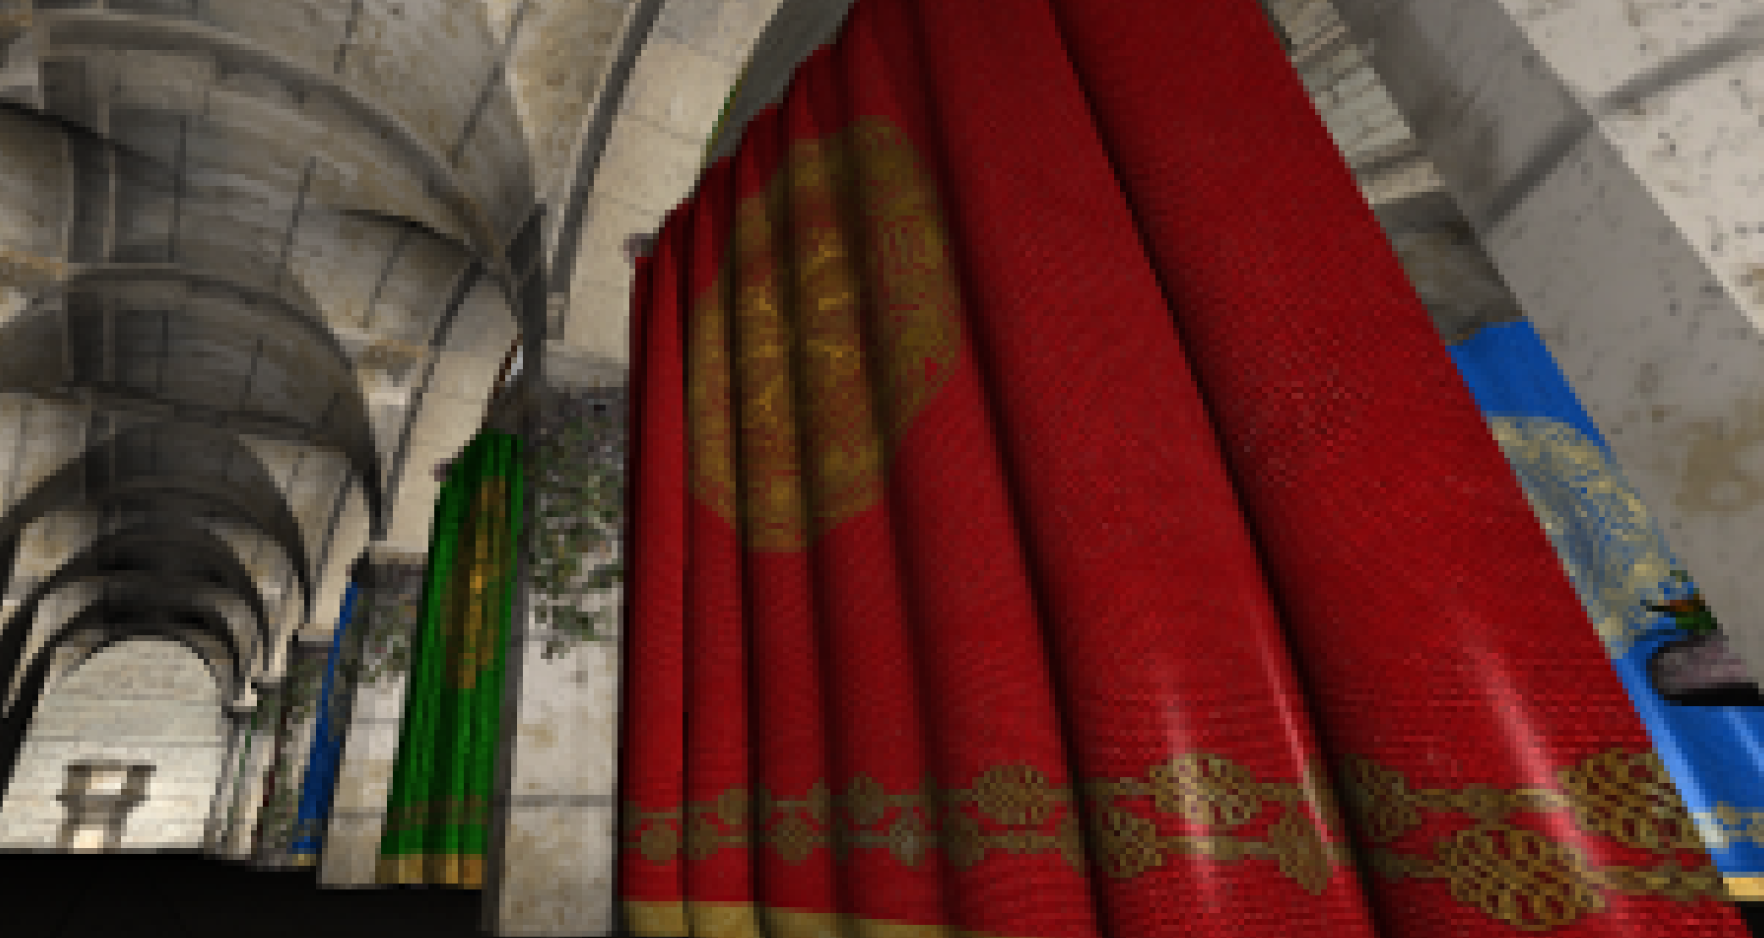
\includegraphics[height=4.0cm,keepaspectratio]{./images/no_transparency.png}}
\hfill % <-- Seperation
\subcaptionbox{Transparent}{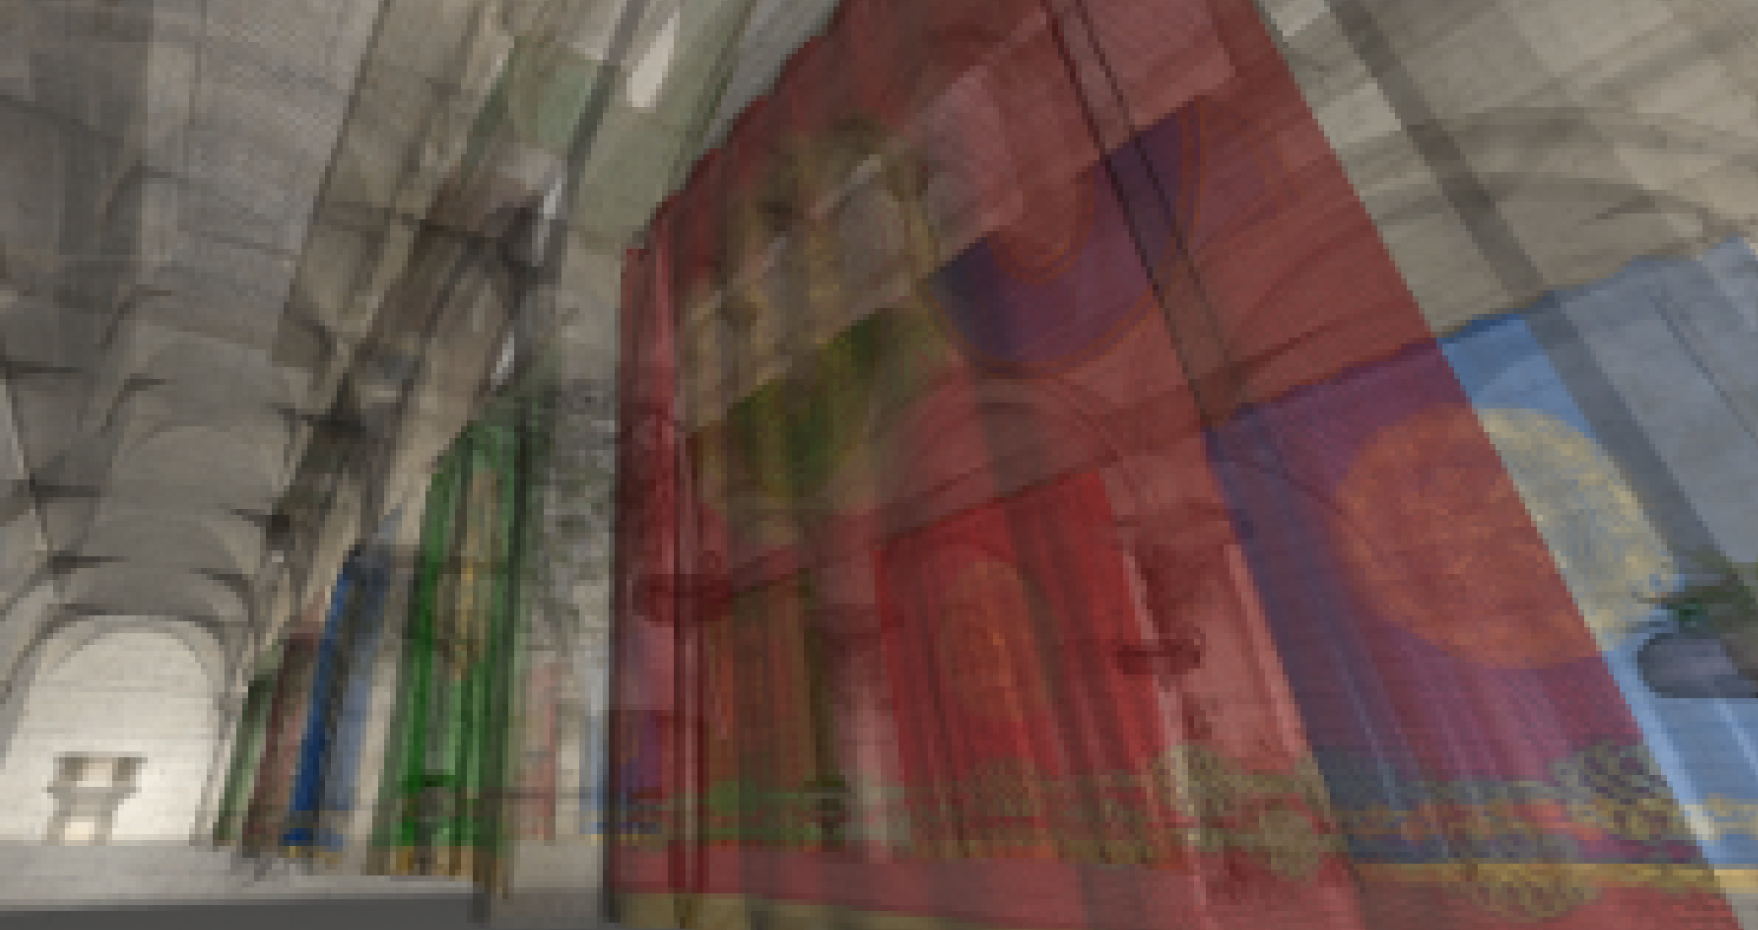
\includegraphics[height=4.0cm,keepaspectratio]{./images/transparency.png}}
\caption{Scene rendered with and without transparency. Taken from \cite{Arch2015}}
\label{fig:Transp}
\end{figure}

A related kind of problem arises in the area of computer graphics \cite{Arch2015}, where on the display of computer generated scenes, each object or polygon to be rendered requires multiple computations to be made as quickly as possible to achieve faster graphic rendering, preferably at real time rates. One of these calculation is the transparency value for each polygon in each pixel that screen is displaying (Figure \ref{fig:Transp}). If we considered that nowadays a screen usually holds millions of pixels, therefore millions of calculations need to take place to run a technique called order independent transparency or OIT, which for each pixel must sort each list in depth order before the transparency operation can be performed. The current approach is to sort them by brute force, meaning that all of the lists are sorted independently.

This problem has been studied, but not in great length, where most of the solutions involves parallel sorting with multi-threading in CPU \cite{han2002integer} and in GPU \cite{hou2017fast},  implementing hybrid algorithms combining the merging power of Mergesort with the speed of comparison based algorithms, like Insertionsort. 
\\

This research then aims to explore if there is other approaches that could aid in the performance in sorting many similar list by taking advantage of potential repetition of elements by using memoization, which is a technique to utilise pre-calculated results, in this case the sorted lists. This involves generating a signature to uniquely identify a repeated list, by using the best suited hash function to produce it.
\\

Due to time constraint during the design and development of this study, an abstraction of the original problem is being studied provided with synthetic data, in a way that it allows to simulate the behaviour of this techniques in different scenarios of the similarity between lists. In order to accomplish this, a testbed was developed that allowed the generation of different sets of data, according to the case that needed to be studied to outline the cases in which the potential of memoization on this problem could be of an advantage over the brute force approach.

\subsection*{Research Questions}
Memoization (see \ref{memoHash}) is a optimisation method used in divide and conquer that consists in the storage of the result of a computation for a later utilisation when the same sub problem arises. This gives better performance because it saves the computation of the same sub problem. To achieve this the result must be stored, generally in a lookup table. Dynamic programming uses this kind of memoization to solve problems based in previous results. For our study, we will use a hash table that will hold the signature of a single list as the key and the reference to the sorted list as the value. The aim therefore is not to determine if this techniques optimises the problem, just because it is always faster performing the sorting operation only once, but to determine when does this technique has a better performance given the overhead of calculating the signature and looking up for the presence of the pre calculated value.\\

This work addresses the following research questions:

\begin{itemize}
\item {\bf RQ1:} What are the benefits of utilising memoization techniques to improve repeated list sorting? When does it happen?
\item {\bf RQ2:} What are the benefit of utilising memoization techniques to improve list sorting when there is repeated blocks within similar lists? When does it happen?
\item {\bf RQ3:} Which hash function fits better to produce a signature over a list of integers?
\item {\bf RQ4:} What are some posibles enhancement techniques that can be applied to improve memoization in sorting?
\end{itemize}

\section{Background}

The problem that is being explored in this research is not the focus of many studies, as there is no direct study on the problem of sorting many similar small list. This might be because the problem is not that common or there has not been a need to optimise this process. For this study we do consider the different areas that are involved in the objectives or that could be of interest to address the questions.

\subsection {Sorting Lists}
The kind of algorithms for sorting can be grouped in different categories, with one of them being the internal sort. These are the kind of algorithms that work with all the data within the main memory through out the whole process.
\begin{itemize}
\item {\bf Insertionsort:}  In this category, {\it Insertionsort} is a simple comparison sorting algorithm that has an average and worse case time complexity of O(${n}^2$), but its best case scenario is O(n). Although it has a poor performance for large lists, we will study it because of its good performance in small lists. Being a stable algorithm, mainly because it sorts the elements in place, using only one auxiliary space in memory\cite{knuth1997artInsert}. Compared to other comparison sorting, like Selectionsort and Bubblesort, all have the same time complexity but in practice the efficiency of this algorithm in the average case is superior to the other quadratic algorithms because there are less comparisons steps. Optimisations over this algorithms have been made, such as Shellsort\cite{knuth1997artShell}, Librarysort\cite{bender2006insertion} and also is part of hybrid algorithms as Timsort\cite{Timsort}.

\item {\bf Mergesort:} The approach of this stable algorithm is sorting by divide and conquer, this by merging the result of the subsequent division of the input list into sub lists and recursively dividing and merging them. The standard implementation uses O(n) in space complexity and has average, best and worst case of O(n logn) in time complexity \cite{knuth1997artMerge}. It is suitable for medium and large data set. Multiple optimisations has been made, mainly to reduce the space complexity and the cost of copying \cite{Huang:1988:PIM:42392.42403}.  Other optimisation takes advantage of the nature of the divide and conquer process, by parallelising the execution with multiple threads \cite{chhugani2008efficient} on different architectures and cache optimised versions. Also it is extensible to be used in external sorting.
 \end{itemize}

Even though these are some of the most popular and studied algorithms, for some cases there are better tuned algorithms suited for specific data, like the one proposed by \cite{han2002integer}  which sort integers and has {$O(n \sqrt{log log n})$} time and space complexity for average cases.

\subsection {External Sort}
External sorting is used when the data to be sorted is too big to fit in main memory so it must be read from the source (network, hard drive) in separate chunks or segments that fits in internal memory. This kind of solution generally apply a hybrid approach in the sorting of the data in memory and merging the final result. 

\subsection{Segmented sort in GPU} 
In the paper \cite{hou2017fast} a new solution is discussed using the advantage of parallel programming using GPU architecture in order to speed the sorting of segments. The solution proposed is based on data that is naturally segmented, and also the reason why it is interesting for us, the distribution of lengths of this segments tends to smaller ones. The authors then debate over the overhead that using multi threading in GPU and the best way to sort each segment individually. The process that they use is finally clustering each segments in buckets of same size and then sorting each one of them using Bitonic sort \cite{batcher1968sorting} so it can be parallelised in GPU, finally to merge them continuously in memory using GPU registers and warp instructions to speed up the process. It must be noted that their approach does not consider taking advantage from the fact that the segments may have some similarities, as is the purpose of this study.

\subsection{Memory Heriarchy}
As much of the literature reviewed exposed, when studying an algorithm not only the time complexity must be taken to account for the performance in speed, because the memory and the operations over it have a great impact on the practical implementation. As Figure     \ref{fig:Memory} shows, memory on a modern end user computer follows a hierarchy, where the CPU register is the fastest one, even for multi core architectures. After that comes in the hierarchy the different levels of Cache in the CPU which gradually have more capacity but they are more expensive to read and write to, comparing in speed. When the CPU needs to load a particular memory location, it first checks if the required address is already in the cache (checking starts from the lowest level and continues to the highest one). If the required address is absent in the cache, then it must be loaded from the main memory. Such situation is called a cache miss. Algorithms should be constructed then to avoid cache misses whenever possible. 

\begin{figure}[H]
\centering
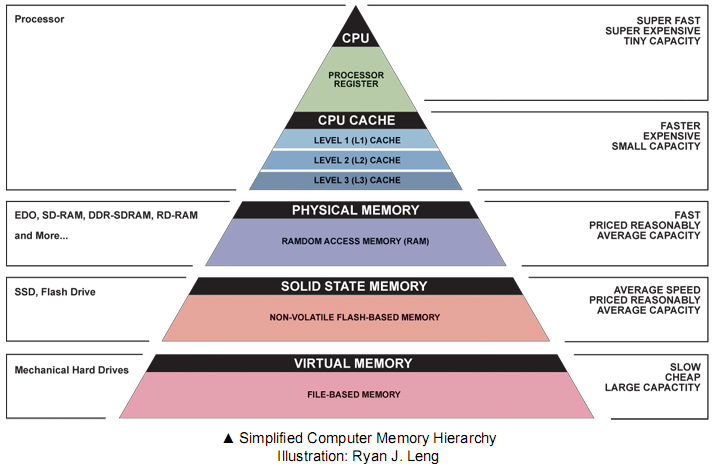
\includegraphics[height=6.5cm,keepaspectratio]{./images/ComputerMemoryHierarchy.png}
\caption{Memory hierarchy. (https://sites.google.com/site/cachememory2011/memory-hierarchy)}
\label{fig:Memory}
\end{figure}

Several modification on known algorithms as Mergesort and Quicksort have been proposed to be {\it cache friendly}, improving the practical performance of such algorithms \cite{lamarca1999influence},  \cite{xiao2000improving}.


\subsection{Memoization and Hashing} \label{memoHash}

Memoization is a concept that has been considered for a long time and has been implemented in different situations \cite{acar2003selective} such as dynamic programming and incremental computation. Most of the applications of this techniques are used to prevent recursive repetition within a function call, to prevent repetition over time, and to
make persistent lookup tables \cite{hall1997improving}. This last approach consists in storing a pair of key and value, and being able to quickly fetch the value given the key if it is present in this table. This property is useful when the calculations to be stored as values are uniquely identified by some key. \\

It is then important for this study to explore the creation of this identity key that could allow us to uniquely map a complete list or a block of the list to be sorted as the key and store the sorted version as the value. \\

Hash functions allows mapping between an undefined set of data to a fixed sized data. Hash functions have many uses, from cryptography, file verification to finding duplicates records. A hash function often needs some type of properties depending on the application of it, because what defines a good hash function could be different if it is used to calculate indexes in a database or to use it as a cryptographic signature. \\

A hash function can be defined as universal if the function itself belong to a family that has the property that the unique value that it evaluates to, h(x), has a probability of 1/M to have two different values x and y to evaluate to the same value, that is h(x) = h(y), which is called a collision. M is the size of all of the possible values the function can return \cite{carter1979universal}.

The classic universal hash function defined in \cite{carter1979universal} is based on a prime number p bigger or equal to M. The constants a and b should be picked from  \{1, p-1\} and  \{0, p-1\} respectively, so to define:

\begin{equation}
    h_{a, b}(x) = ((ax + b)  * mod p) * mod M 
\end{equation}


Furthermore a hash function {\it h} is considered strongly universal if the probability of having two different keys, x and y and the hash function for the event h(x) and h(y) is 1/$M^{2}$. In other words, strong universality is that each key is hashed uniformly into M, and that distinct keys are hashed independently.\\

When the size of the universe of keys is smaller or equals to the possible outcomes (M), there are ways to construct what is known as a perfect hash function  \cite{sprugnoli1977perfect}, where there is no collisions for any given key.  This might be the best solution to construct a lookup table, or hash table, to be able to apply the memoization technique. Given that the universe of the problem we are exploring consists of a pre defined length of lists and the range of the elements in the lists are limited, there should be a hash function that is perfect for this problem, but the size of M might be too big or the performance of it  could be worse compared to a sufficiently strongly universal or even only universal hash function in this particular study.

\subsection{Compiling vs Interpreting code}
When developing a benchmark framework it is important to consider the precise tools for it. Programming languages have the capability to be interpreted or to be compiled, it all depends if there is a compiler or an interpreter available for the specific language. An interpreter is a program that executes the instruction written in the source code by reading each line of code, translating it to machine code and executing it, making the source code the actual program. This allows that any machine that has the correspondingly interpreter can run the program, making it inter operable and also easier to debug. Some of the usual interpreters are build for scripting languages, such as Javascript.

On the other hand, compilers produces code from the source code  reading the whole code and transforming it to assembly language, which is then assembled into binary code and packed into a program. This program can only be executed in the same machine architecture in which it was compiled, making it less portable, but generally is faster than interpreting code because each instruction is executed directly, instead of going through the process of being interpreted each time. Languages such as C or C++ are usually compiled.

There is another hybrid approach, where a runtime environment is provided in the machine where the program is set to run. This environment executes code by interpreting it or determining if some part of the code is heavily used, then it compiles it to later execute the compiled code instead of interpreting it. This is called  just in time compiling or JIT. Some of the languages that provides this environments are Java and Python.

\section{Design and Development}
Given the exploratory objective of this research on the feasibility of using memoization on sorting lists, which by itself is a generalisation of a specific problem, the evaluation considers running each sorting algorithm on the same synthetic data set generated specially to understand the behaviour of it in specific cases. The goal is to measure the amount of time taken to sort the full data set, also considering the amount of memory needed to accomplish it.

\subsection{Synthetic Data}

In order for the data set to be representative of the original problem that this study  took inspiration from, the amount of lists correspond to half of what could be the expected amount of data to be processed. This comes from the fact that the sorting of transparency lists needs to be done for each pixel shown in a physical screen, so considering that nowadays most screen have a HD or Full HD resolution, which display a resolution of 1,920 x 1,080, we have around 2 millions pixels to sort. For the purpose of this study  we will use half of the amount of available pixels (approximately 1 million) because it provides a good enough representation of a real case scenario but it still allows to run test in a environment without exceeding system memory or CPU specification.

Each of the million lists to be tested is generated to hold uniformly distributed random generated integer numbers that range between 0 and RAND\_MAX in C++ (value depends on the implementation, but normally is 2,147,483,647), just  to have a big enough pool to distribute it through the different lengths that are tested, which vary between cases. To generate the baseline on run time between sorting algorithms and also compare them using the new algorithms to use memoization in order to answer RQ1, the length of the lists considered were from 16 integers to 512. For RQ2 to be answered, this is sorting blocks within the lists, a larger length of the lists is needed because of the expected overhead that reading and merging blocks or sublists brings, so for smaller lists no better performance is expected given that it is already fast enough, so increasing the length size permits for an actual appreciation of what could be the benefits of applying this technique.\\

Finally, each array's data is generated accordingly to the scenario that it is being tested. Given that for RQ1 and RQ2 the behaviour that it is studied is on repeating list and similar list, it is then necessary to state how much repeating lists or how similar are them. 

\subsection{Test Cases}

For RQ1 different scenarios will be tested on each array length size. Each scenario is as follow:
\\

\begin{tabular}{|l|l|} \toprule
	{$Repetition $} & {$Description$}  \\ \midrule
	100\% & Only one original list \\
	75\% & 250,000 originals list  \\
	50\% & 500,000 originals list \\
	25\% & 750,000 originals list \\
	0\% & All lists are different \\ \midrule
\end{tabular}

For RQ2 the different scenarios are the following:
\\

\begin{tabular}{|l|l|} \toprule
	{$Repetition $} & {$Description$}  \\ \midrule
	100\% & Only one  original block, repeated for the rest of the data \\
	75\% & 250,000 originals blocks   \\
	50\% & 500,000 originals blocks \\
	25\% & 750,000 originals list \\
	0\% & All blocks are different \\ \midrule
\end{tabular}

For each of this scenarios, different length of blocks will be tested, still to be defined but given the preliminary results, choosing small length blocks will produce an overhead in memory and in operations and choosing a higher block will convert it into a RQ1 scenario. \\

The testbed will be executed in a 2017 MacBook Pro, with a 2.3 GHz Intel Core i5 and 16 GB 2133 MHz LPDDR for physical memory. Compiled by GCC 4.2.1 in macOs Mojave 10.14.4.

%  This only applies for research methods  
%After all this test are executed and analysed, some real data from the inspirational problem could be tested, but some %modification either to the software or the original data set would have to be made, because the data itself is different, as it %works with different size floating points between 0 and 1 and our current approach only works with integers.

\subsection{Hash Function}

In order to consider which hash function to implement, the universe of possible inputs has to be considered. We are only working with sets of integers with elements between 0 and RAND\_MAX, and each list (or a block of it) is a key or input for the hash function. 
Then the size of the universe of keys is the combination of the range of integers over the size of the lists $\binom{RAND\_MAX}{Max list length} $, which in the environment where the test bed will be run, where max list length is 512, it is in the order of $10^{3611}$.

Given this universe size, considering a perfect universal hash function is impossible because the potential hash table needs $10^{3611}$ elements to map to. In consequence, a strongly universal hash function will be considered.

As reviewed by \cite{thorup2015high}, one of the fastest technique to construct a strongly universal hash function for an integer set is to multiply and shift pairs of elements, given the following formula:

\begin{equation}
	h_{a_0,a_{d-1},b} (x_0, x_{d-1}) = \Bigg(\Bigg( \sum_{i=0}^{d/2} (a_{2i} + x_{2i+1})  (a_{2i+1} + x_{2i})\Bigg)  + b\Bigg) [W-l, W).
\end{equation}

Where {\it d}  is the length of the set and it is assumed to be even. The set {\it a} is a set of uniformly random distributed integers in the  range $[0,2^w]$ where w is the amount of bits of the keys,{\it b}  is just a constant in the range $[0,2^w]$. The seed {\it l}  is the bits of the hash value. {\it W}  is at least the sum of w + l -1 or higher. \\
Then the hash function proposed is named {\bf PairMultiplyShift}, and has the following pseudo-code:

\begin{verbatim}
int hash(int[] data, int l, int[] a, int b, int w, int d) {
    hash = 0;
    for(int i = 0; i < d/2; i++) {
        pairResult =  (a[2i] + data[2i+1]) * (a[2i+1] + data[2i]);
        hash +=  (pairResult + b) >> (w-l);
    }
    return hash;
}
\end{verbatim}

For our case, the keys used are 32 bit integers (4 bytes) and the algorithm involves multiplication then we need to handle 64 bits results, so in order to maintain a low probability of collisions and taking advantage that the 64 bit multiplication automatically discards overflow,  the hash value is defined as 64 bits (8 bytes)
\\

It is then stablished that this kind of hash function has a time complexity of O(n) and space complexity of O(l). For educational purpose and to understand the impact of choosing the correct hash function, other hash functions are also tested, even though it is known before hand that some of them are not the best solution to the problem.

The following hash function are compared:

\begin{itemize}

\item {\bf MD5:} This is a cryptographic function \cite{rivest1992md5} which is no longer secure \cite{wang2005break}.  The implementation is given by the standard C++ library {\it CommonCrypto}.

\item {\bf PrimeAdd:} The naive approach of just adding the value of each element and multiplying by a prime number. The objective is to do simple operations, multiplication and addition, and exploiting the know properties of prime numbers of producing number with less common factors. \\ 
The proposed algorithm is:

\begin{verbatim}
int hash(int list[], int length) {
 long hashVal = 17;
    for(int i = 0; i < length; i++) {
        hashVal = hashVal * 19 + list[i];
    }

    return to_string(hashVal);
}
\end{verbatim}
 

\item {\bf MurMur3:} A non-cryptographic hash function suitable for general hash-based lookup. Implemented based on the source code available online \cite{MurMur3}. This hash function works by rotating, shifting and Xoring chunks of bytes. It provides 3 methods, 1 for hash values of 32 bits and 2 for 128 bits (for x86 and 64 bits architectures). The one used is MurmurHash3\_x64\_128, but 64 of the 128 bits are discarded to maintain the same value to compare to other functions.

\end{itemize}

\subsection{Implementation of Insertionsort and Mergesort}
It is important to discuss the implementation of the sorting algorithms as it impacts directly on the performance and the extensibility of it.

For Insertionsort, the implementation used is the straight forward iterative approach, comparing tuples starting from the second position and moving to the end of the list. The implementation is as follows:

\begin{figure}[H]
\begin{small}
\begin{verbatim}
void InsertionSort::sort(int list[], int length) {
	int value;
	int i, j;
	for(i = 1; i < length; i++) {
	    value = list[i];
	    j = i-1;

	    while (j >= 0 && list[j] > value) {
	        list[j+1] = list[j];
	        j = j-1;
	    }
	    list[j+1] = value;
	}
}
\end{verbatim}
\end{small}
\caption{Insertionsort implementation}
\end{figure}


The case for Mergesort is more interesting, because the natural approach is to have depth first  recursive calls. The way that was implemented in this study is by bottom up approach, which is an iterative double loop that operates in place and merges the arrays in pair, doubling the range of each tuple in each loop. The advantages for this choice of implementation is to avoid the recursive function call overhead and the ability to access in place to all elements, which gives the opportunity for further modifications when considering memoization over the algorithm.

\begin{figure}[H]
\begin{small}
\begin{verbatim}
void MergeSort::mergeSort(int list[], int length) {
   for(int mergingArraySize = 1; mergingArraySize < length;
    		mergingArraySize = (2 * mergingArraySize)) { 

       for(int startIndex = 0; startIndex < length-1; 
       		startIndex += (2 * mergingArraySize)) { 
           int half = startIndex + mergingArraySize - 1; 
           int endIndex = min((startIndex + (2 * mergingArraySize) - 1), length-1);

           merge(list, startIndex, half, endIndex); 
       } 
   } 
}

void MergeSort::merge(int list[], int startIndex, int half, int endIndex) {
  int leftListLength = half - startIndex + 1; 
  int rightListLength = endIndex - half; 

  for(int i = 0; i < leftListLength; i++) {
    leftList[i] = list[startIndex + i]; 
  }

  for(int i = 0; i < rightListLength; i++)  {
    rightList[i] = list[half + 1 + i]; 
  }

  int i = 0;
  int j = 0;
  int globalIndex = startIndex; 

  while (i < leftListLength && j < rightListLength) { 
      if (leftList[i] <= rightList[j]) { 
          list[globalIndex] = leftList[i]; 
          i++; 
      }  else { 
          list[globalIndex] = rightList[j]; 
          j++; 
      } 
      
      globalIndex++; 
  } 
  
  while (i < leftListLength) { 
      list[globalIndex] = leftList[i]; 
      i++; 
      globalIndex++; 
  } 
}
\end{verbatim}
\end{small}
\caption{Mergesort bottom up implementation}
\end{figure}

\subsection{Hash table: Unordered map} \label{hashTable}
As stated before, the selected underlying hash table used to store the signature is the one offered as part as the containers library in c++ named unordered\_map, which is a structure that holds the pair (key, value) and it has O(1) in the average case for the search, insert and delete operation.

This hash table expands automatically because it keeps count of the amount of items holding and grows it size and rehash all elements when it reaches the load factor, which is the ratio between the number of elements and the size of the hash table. 
\begin{figure}[H]
\centering
\subcaptionbox{Insertion}{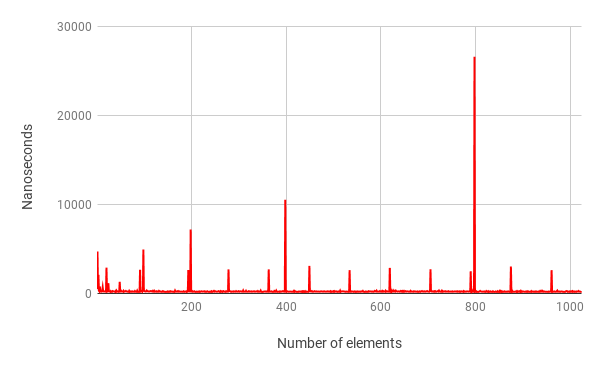
\includegraphics[height=4.5cm,keepaspectratio]{./images/insertHashTable.png}}%
\hfill % <-- Seperation
\subcaptionbox{Look up}{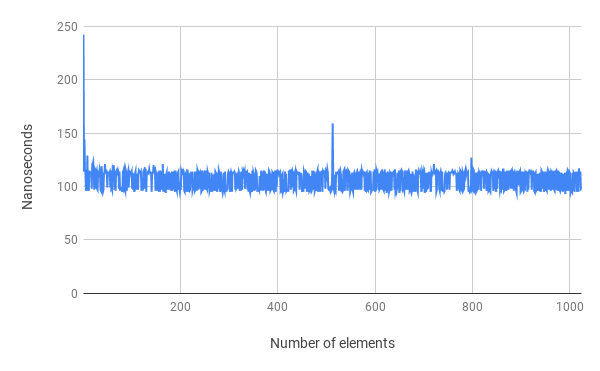
\includegraphics[height=4.5cm,keepaspectratio]{./images/searchHashTable.png}}%
\caption{Unordered map operations}
\label{fig:hashTableFig}
\end{figure}

Empirically the operations of insertion and look up values can be viewed in Figure \ref{fig:hashTableFig}, where 1024 random integers were inserted and immediately searched. The insertion operation have spikes that are bigger as the hash table is filled, which is explained by the resizing process explained before. 

It can be viewed that both insertion and search operation generally maintains a constant time.

\subsection{MemoSort for repeating lists}
To be able to take advantage of the possible repeating nature of the problem being studied we use the described hash table and hash function to implement a memoization technique. We propose \textbf{MemoSort} which is the algorithm being studied to establish its real benefits, and its defined by the following pseudo algorithm: 

\begin{figure}[H]
\begin{small}
\begin{verbatim}
for(j = 0; j < listLength; j++) {
    signature = hashFunc.hash(lists[j]);  // Generates signature for list
    sortedListIndex = hashTable.find(signature) // Look signature in hash table
    
    if(sortedListIndex not found) // New list to be sorted
         sortFunction.sort(lists[j]); // Sorts list
         hashTable.insert(signature, j); // Stores the reference to the sorted list
     } else  // List already sorted
        lists[j] = lists[sortedListIndex] // Copy sorted list
}
\end{verbatim}
\end{small}
\caption{MemoSort pseudo algorithm}
\end{figure}

The theoretical behaviour for each of the sorting algorithm gives us an idea on the amount of overhead that the construction and  execution of the look up in the hash table has to take. 

For Insertionsort, the worst time complexity is O($n^2$), being n the length of the list and if M is the total amount of lists to sort in brute force case, and M$'$ the amount of unique lists to sort when using memoization, then it follows that:

\begin{equation}
M * O_{sorting}(n^2)  \geq M' * O_{sorting}(n^2)  + Overhead
\end{equation}
Which implies
\begin{equation}
(M - M') *  O_{sorting}(n^2)  \geq Overhead
\end{equation}

As the memoization technique involves the operation for each list of calculating the signature, looking up each, and insert only the ones that are unique, then:

\begin{equation}
Overhead =  M * O_{hashing} + M * O_{lookup} + M' * O_{insert}
\end{equation}

Accordingly the implementation of the hash table then has to be constant for both the search of a key and in the insertion of a new tuple. Other operations as delete or edit are of no concern because they do not apply for the use of this memoization technique. Then constructing the hash table is a matter of using the correct data structure. For this case the choice was to use an unordered map (see \ref{hashTable}). Other options involves the usage of trees, which have O(n logn) operations.
\\
In consequence for the memoization technique to be beneficial it must stand that:

\begin{equation}
(M - M') *  n^2  \geq M * O_{hashing} + M'
\end{equation}

From this, the following cases can be defined:
\begin{itemize}
\item {\bf All lists are the same:}  This means M$'$ = 1, holds clearly that (M - 1) *   $O_{sorting}(n^2)$   $\geq M *O_{hashing}(n)$ + 1
\item {\bf None of the lists are the same:} This means M$'$ = M. Then there is no benefit as 0 $ \geq M * O_{hashing}(n)$ + M is not true if M $>$ 0
\end{itemize}

The same analysis can be made for the case of Mergesort where sorting is for worst case is O(n logn). \\

\subsection{MemoSort optimised for repeating lists}
The intuition to this approach comes from the fact that when sorting there is the need to visit each element at least once, as in the current approach of calculating the signature, so merging both process may result in a faster approach.
For each case the hash table holding the current calculated signatures need to be passed as a reference to the sorting method and queried as soon as the signature is calculated. If the signature is not present, the signature is stored in the hash table with the reference to the ordered list. \\

In Insertion sort, only after half of the array is processed the signature can be calculated, so it saves at least half of the operations. Different is the case of Mergesort where after the first pass of the merge step all elements have been visited and the signature can be calculated, thus saving al the subsequent merging steps.

\subsection{MemoBlockSort for similar lists}
* Define pseudo algorithm

\subsection{MemoBlockSort optimising by K-merging}
* Define pseudo algorithm

\subsection{MemoBlockSort optimising by 2-merging}
* Define pseudo algorithm

\subsection{MemoBlockSort optimising by 4-merging}
* Define pseudo algorithm

\subsection{Optimising by use of memory for similar lists}
* Define ways to improve the code to use less memory

\subsection{MemoBlockSort optimising for ordered blocks}
* Define pseudo algorithm

\section{Results}
\subsection{Benchmarking}

The first activity that was developed was to design and build a software framework that could guarantee correct and trustworthy calculation of the execution of certain algorithms. The first approach was to develop the software in Java language version 8, but it proved to be a not so reliable language for benchmarking given that the Java Virtual Machine environment on which the program runs, uses JIT  compilation and handles memory through a garbage collector in a unpredictable way, thus when running the experiments the results vary in a big percentage. The first measure to mitigate this was to run each test ten times and calculate an average on the result. Also, to prevent the compilation of code throughout the test, the code had to be {\it warmed up} by executing it a number of times so it would be forcefully compiled. 

Even after taking this safeguarding, the tests took a long time to run, and still the results were not as solid as it is required to confidently compare algorithms. For that reason, the code was re written in C++. With this new code the test where  executed and it prove to give more concise and uniform results. This allowed to execute the test a couple of times without having a big difference (below 0.5\%), having consistent result in overall, so the results presented are just the execution of a single test.

\subsection{Mergesort vs Insertionsort}

\begin{figure}[H]
    \centering
     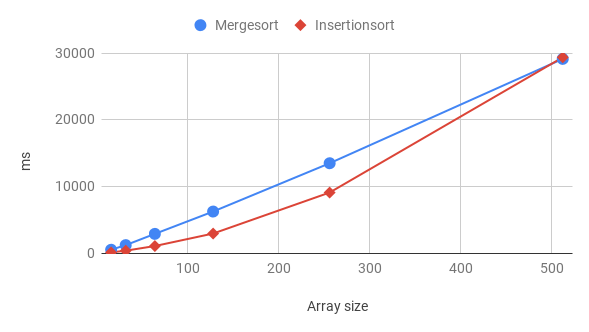
\includegraphics[height=8cm,keepaspectratio]{./images/InsertionvsMerge.png}
    \caption{Insertionsort v/s Mergesort}
    \label{fig:InsrtVsMerge}
\end{figure}

The first experiment executed was to compare algorithms Insertionsort and Mergesort given the synthetic data set created, which comprehends all three scenarios (worst, best and average) using the same parameters for each one. As the literature confirms, Insertionsort has a better performance on smaller length list. By using the parameter $-o2$ to compile the code, better results are obtained and Insertionsort sorts in less time until length of 512 elements. After this length of list, Mergesort has a better performance.

The time taken to sort the lists in milliseconds is displayed in Figure \ref{fig:InsrtVsMerge}. Only the average case (random order) for both algorithms are displayed and they exhibit the expected behaviour, this is  O(${n}^2$) for sorted array in Insertionsort and O(n logn) time complexity for Mergesort. This is explained because Insertionsort performs less operations and most importantly has less read and write operations over the array. In contrast, merge sorts reads and writes through the data for each merge, making it more expensive to sort when the overhead of this operations takes almost all the time of the sorting, which happens when the amount of elements is small.

\subsection{Hash functions}

\begin{figure}[H]
    \centering
    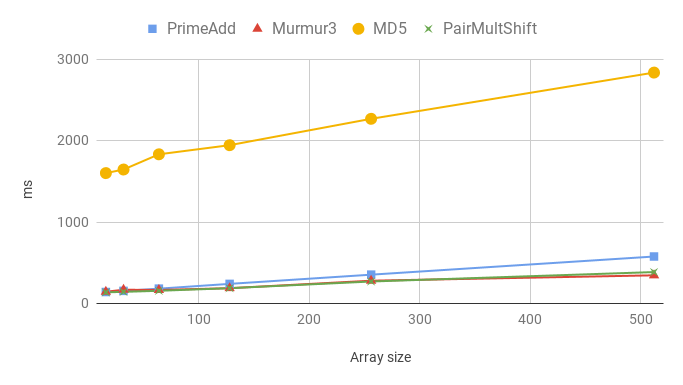
\includegraphics[height=8cm,keepaspectratio]{./images/hashes.png}
    \caption{Hash functions comparison}
    \label{fig:HashesFunc}
\end{figure}

From Figure \ref{fig:HashesFunc} is it clear that all hashing function have a linear behaviour, but they do show performance differences between them. It is visible that MD5 is not a viable hash function to use for this study because of the time it takes compared to the other functions, being orders of magnitude of difference. This confirms that this functions is not designed for use in a hash table.

Then comparing the other three hash functions, {\it PrimeShift} hash function behaves as wells as the others two, but it begins to be slower after the array length is bigger than 64 elements. The difference continues to increase as there are more elements in the lists.

Both {\it Murmu3} and {\it PairMultShift} behave in a similar way, growing by a really small amount and having a small difference between them, that could be part of the randomness of the tests. Both approaches are radically different but behaves as well for arrays of integers.

It must be stated that all of the functions presented 0 collisions for each of the runs.

TODO: Compare memory.


\subsection{MemoSort for repeating lists}

In order to better compare what is the performance of the memoization techniques, a base cost must be stablished in the use of a hash table, by determining the time spent inserting and searching from it. An experiment was conducted to determine how much time did it take in the operation of inserting all possible signatures, and how much time did it take to search for one after the hash table was full:

\begin{itemize}
\item Inserting all signature: 823 milliseconds
\item Searching for one signature in full table: 257 nanoseconds
\end{itemize}

The following result represent the test over uniformly distributed random data after applying the memoization technique using a hash table, and using the selected hash function to generate the signature of each of the unique list. \\

\begin{figure}[H]
\centering
\subcaptionbox{0 repetition}{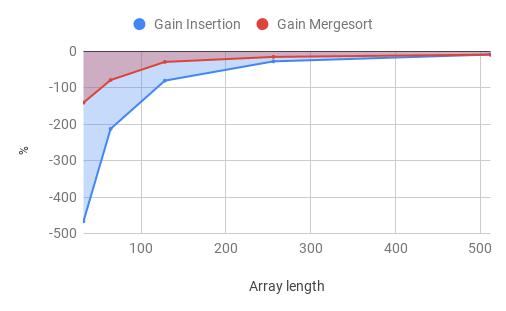
\includegraphics[height=4.3cm,keepaspectratio]{./images/list_0_repeat.png}}%
\hfill % <-- Seperation
\subcaptionbox{25\% repetition}{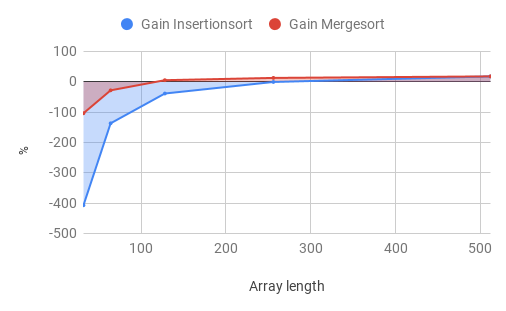
\includegraphics[height=4.3cm,keepaspectratio]{./images/list_25_repeat.png}}%
\\ % <-- Line break
\subcaptionbox{50\% repetition}{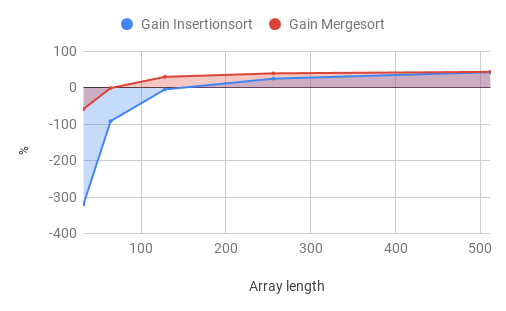
\includegraphics[height=4.3cm,keepaspectratio]{./images/list_50_repeat.png}}%
\hfill % <-- Seperation
\subcaptionbox{75\% repetition}{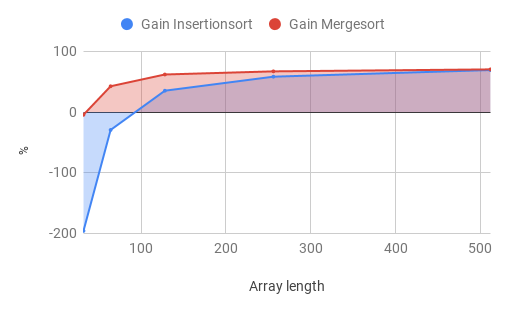
\includegraphics[height=4.3cm,keepaspectratio]{./images/list_75_repeat.png}}%
\\ % <-- Line break
\subcaptionbox{100\% repetition}{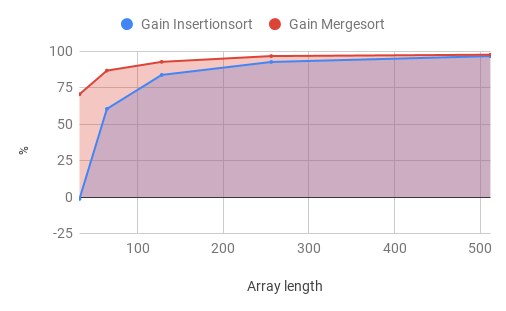
\includegraphics[height=4.3cm,keepaspectratio]{./images/list_100_repeat.png}}%

\caption{Memoization performance}
\label{fig:MemPerfRepeat}
\end{figure}


The results displayed in Figure \ref{fig:MemPerfRepeat} shows the performance comparison in a ratio to the case of brute force sorting all list for each algorithm with uniform random data, where it can be seen that there is a severe penalty for using this approach in small length lists for Insertionsort. There starts to be an improved performance after lists with length of 128, mainly because the sorting performance below this length surpass the overhead of calculating and looking up the signature of the list. \\
As it is expected, when there is no repetition, there is only overhead in applying this approach. The trend tends to be that the bigger the list length, the more gain there is. Can be concluded the that in a general case, there is a gain when there is 50\% or more list repetition.

The same behaviour is shown for Mergesort, but the gain is not given much by the length of the array, as only for the amount of repeated lists given that the increase or decrease is not so drastic as with Insertionsort.

\subsection{MemoSort Optimisation for repeating lists}

\subsection{MemoBlockSort in similar lists}

TODO
\begin{itemize}
\item Graph of time for each approach
\item Table of memory.
\end{itemize}

\section{Conclusions}

TODO
\begin{itemize}
\item Conclusion on hash functions (it depends on the data, even on the architecture of the computer) but using generic but proven universal hash function is a better approach if the data is not known before hand, where a perfect hash function is preferred.
\item Conclusions of Memoization in repeating lists (It has gain starting from 50\% repetition), compared to optimised sort is better.
\item  Conclusions of Memoization in similar lists ?.
\end{itemize}

\section{Future Work}

While the objectives of this study serves as a initial exploration and they are reached by running the test cases with synthetic data, there is a need to find a suitable problem where the nature of the data fits the conclusions, so it can benefit of  the explored memoization techniques. The problem that served as inspiration \cite{Arch2015} is a possible candidate but some changes need to be done to fit the data of this problem, further more, some preliminary probing suggest that the data is not so repetitive to be able to benefit from the techniques studied.

Because the limitation on time of this study, there are multiple different improvements or alterations to be made to test the techniques in different scenarios, like exploring the behaviour with cache friendly version of the sorting algorithms and using the power of parallelisation by multi threading in CPU or by implementing memoization techniques in GPU sorting.

Also other memoization techniques can be constructed, like a probabilistic heuristic that samples elements of the lists between lists, instead of reading the whole list to match for previous sorted list.

For the specific problem on choosing the correct hash function, from the multiple implementations of hash functions, there may be faster one that is not universal but still have no collisions within the problems data and makes the memoization techniques more beneficial.

Other approaches to determine the similarities between list can be explored other than using a hash table, like local sensitive hashing, specifically the MinHash algorithm which can determine with a hash function the similar sets with a percentage of error.

\bibliographystyle{alpha}
% there are various bibliography styles you can set

\bibliography{references}
% this tells latex to generate the reference list, using the references.bib file of references.
% you will need to do pdflatex <tex filename>; then bibtex <tex filename without extension>;
% pdflatex <tex filename> again twice. then you have a formatted pdf.

\section{Apendix}

\end{document}
